% Für Bindekorrektur als optionales Argument "BCORfaktormitmaßeinheit", dann
% sieht auch Option "twoside" vernünftig aus
% Näheres zu "scrartcl" bzw. "scrreprt" und "scrbook" siehe KOMA-Skript Doku
\documentclass[12pt,a4paper,headinclude,bibtotoc]{scrartcl}


%---- Allgemeine Layout Einstellungen ------------------------------------------

% Für Kopf und Fußzeilen, siehe auch KOMA-Skript Doku
\usepackage[komastyle]{scrpage2}
\pagestyle{scrheadings}
\automark[section]{chapter}
\setheadsepline{0.5pt}[\color{black}]

%keine Einrückung
\parindent0pt

%Einstellungen für Figuren- und Tabellenbeschriftungen
\setkomafont{captionlabel}{\sffamily\bfseries}
\setcapindent{0em}

\usepackage{caption}

%---- Weitere Pakete -----------------------------------------------------------
% Die Pakete sind alle in der TeX Live Distribution enthalten. Wichtige Adressen
% www.ctan.org, www.dante.de

% Sprachunterstützung
\usepackage[ngerman]{babel}

% Benutzung von Umlauten direkt im Text
% entweder "latin1" oder "utf8"
\usepackage[utf8]{inputenc}

% Pakete mit Mathesymbolen und zur Beseitigung von Schwächen der Mathe-Umgebung
\usepackage{latexsym,exscale,amssymb,amsmath}

% Weitere Symbole
\usepackage[nointegrals]{wasysym}
\usepackage{eurosym}

% Anderes Literaturverzeichnisformat
%\usepackage[square,sort&compress]{natbib}

% Für Farbe
\usepackage{color}

% Zur Graphikausgabe
%Beipiel: \includegraphics[width=\textwidth]{grafik.png}
\usepackage{graphicx}

% Text umfließt Graphiken und Tabellen
% Beispiel:
% \begin{wrapfigure}[Zeilenanzahl]{"l" oder "r"}{breite}
%   \centering
%   \includegraphics[width=...]{grafik}
%   \caption{Beschriftung} 
%   \label{fig:grafik}
% \end{wrapfigure}
\usepackage{wrapfig}

% Mehrere Abbildungen nebeneinander
% Beispiel:
% \begin{figure}[htb]
%   \centering
%   \subfigure[Beschriftung 1\label{fig:label1}]
%   {\includegraphics[width=0.49\textwidth]{grafik1}}
%   \hfill
%   \subfigure[Beschriftung 2\label{fig:label2}]
%   {\includegraphics[width=0.49\textwidth]{grafik2}}
%   \caption{Beschriftung allgemein}
%   \label{fig:label-gesamt}
% \end{figure}
\usepackage{subfigure}
\usepackage{adjustbox}

% Caption neben Abbildung
% Beispiel:
% \sidecaptionvpos{figure}{"c" oder "t" oder "b"}
% \begin{SCfigure}[rel. Breite (normalerweise = 1)][hbt]
%   \centering
%   \includegraphics[width=0.5\textwidth]{grafik.png}
%   \caption{Beschreibung}
%   \label{fig:}
% \end{SCfigure}
\usepackage{sidecap}

% Befehl für "Entspricht"-Zeichen
\newcommand{\corresponds}{\ensuremath{\mathrel{\widehat{=}}}}

%Für chemische Formeln (von www.dante.de)
%% Anpassung an LaTeX(2e) von Bernd Raichle
\makeatletter
\DeclareRobustCommand{\chemical}[1]{%
  {\(\m@th
   \edef\resetfontdimens{\noexpand\)%
       \fontdimen16\textfont2=\the\fontdimen16\textfont2
       \fontdimen17\textfont2=\the\fontdimen17\textfont2\relax}%
   \fontdimen16\textfont2=2.7pt \fontdimen17\textfont2=2.7pt
   \mathrm{#1}%
   \resetfontdimens}}
\makeatother

%Si Einheiten
\usepackage{siunitx}

%c++ Code einbinden
\usepackage{listings}
\lstset{numbers=left, numberstyle=\tiny, numbersep=5pt}

%Differential
\newcommand{\dif}{\ensuremath{\mathrm{d}}}

%Boxen,etc.
\usepackage{fancybox}
\usepackage{empheq}

%Fußnoten auf gleiche Seite
\interfootnotelinepenalty=1000

%Dateien aus Unterverzeichnissen
\usepackage{import}

%Bibliography \bibliography{literatur} und \cite{gerthsen}
%\usepackage{cite}
\usepackage{babelbib}
\selectbiblanguage{ngerman}

\begin{document}

\title{Navigation}
\author{Felix Kurtz}
\maketitle

\section{GPS Versuch}
Das Satelliten-Navigationssystem \textsc{GPS} beruht darauf, dass man von drei bzw. wegen relativistischen Effekten vier bekannten Positionen durch Abstandsmessungen zu einer unbekannten Position diese bestimmen kann.
Dabei wird der Abstand über die Laufzeit der Photonen bestimmt, denn diese bewegen sich mit konstanter Geschwindigkeit, der Lichtgeschwindigkeit.
In diesem Versuch soll dies 

Aus der Differenz von Start- und Zielzeit wird die Wegstrecke der menschlichen Photonen bestimmt.
\begin{table}[!htb]
	\centering
	\begin{tabular}{|c|c|c|c|c|c|}
		\hline		
		Position & Startzeit & Zielzeit & Dauer $\Delta t$ & $v^{-1}$ & Strecke $\Delta s$\\
		\hline
		Schranke & 15:26:00 Uhr & 15:26:39 Uhr & $39\,$s & $8.86 \frac{\si{\second}}{10\si{\meter}}$ & $44\,$m\\
		Brücke & 15:25:57 Uhr & 15:26:52 Uhr & $55\,$s & $9.78 \frac{\si{\second}}{15\si{\meter}}$ & $84\,$m\\
		Haus 21 & 15:27:20 Uhr & 15:28:15 Uhr & $55\,$s & $10.5 \frac{\si{\second}}{15\si{\meter}}$ & $79\,$m\\
		\hline
	\end{tabular}
	\caption{GPS-Versuch: Messdaten}
\end{table}

\begin{figure}[!htb]
	\centering
	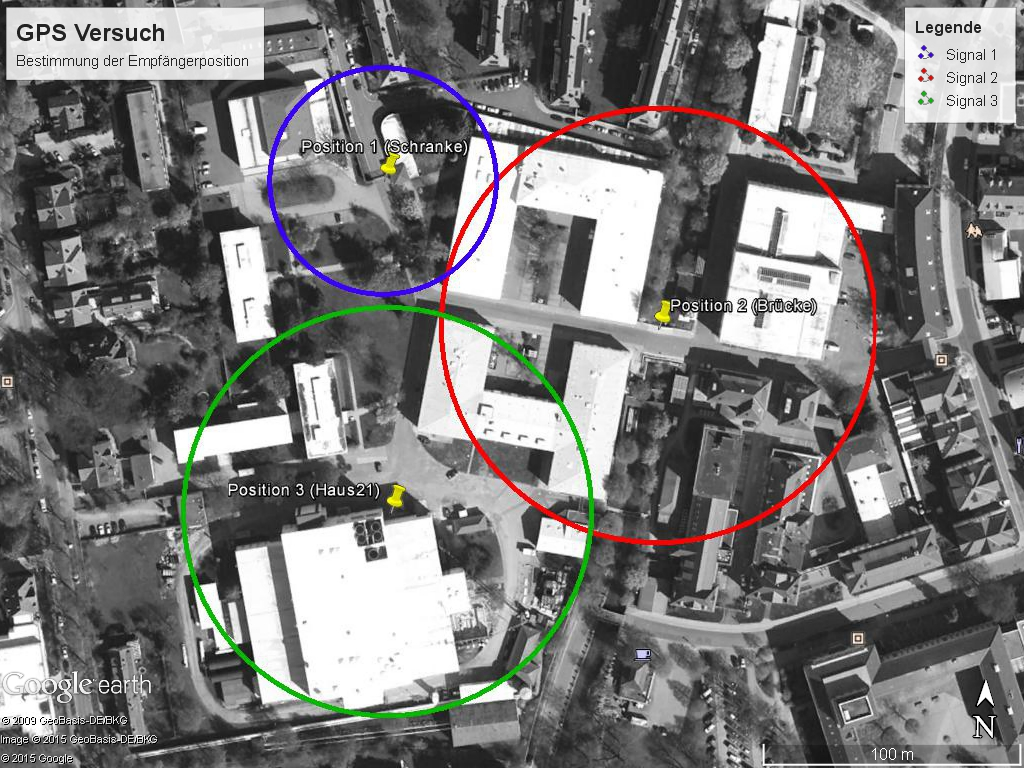
\includegraphics[width=0.8\textwidth]{GPS.jpg}
	\caption{Karte des DLR-Geländes mit den drei Satellitenpositionen und zugehörigen}
	\label{fig:gps}
\end{figure}

\section{Foucaultsches Pendel}
Zuerst bestimmt man mit einem Pendel die Erdbeschleunigung $g$:
Für den Tangentialanteil der Gewichtskraft gilt nach Newton: $F_{G,\text{tan.}}=mg \ddot{\varphi}$.
Für kleine Winkel ist er etwa linear zur Auslenkung: $F_{G,\text{tan.}}\approx mg\varphi$.
Die sich daraus ergebende Differentialgleichung lässt sich z.B durch $\varphi(t)=A\cos(\omega t)$, mit der Amplitude $A$ und der Kreisfrequenz $\omega=\sqrt{\frac{g}{l}}$ lösen.
Daraus lässt sich die Periodendauer
\begin{align}
	T =\frac{2\pi}{\omega}= 2\pi \sqrt{\frac{l}{g}}
\end{align}
bestimmen bzw. aus ihr die hier gesuchte Erdbeschleunigung (inklusive Fehlerformel aus der Gaußschen Fehlerfortpflanzung)
\begin{align}
	g &= 4\pi^2 \frac{l}{T^2}\,,\\ \label{eq:gbesch}
	\sigma_g &= \frac{4\pi^2}{T^2} \sqrt{\sigma_l^2+\left(\frac{2l}{T}\right)^2 \cdot\sigma_T^2}
\end{align}
ausrechnen.
Da diese nicht von der Pendelmasse abhängt, wird nur die Seillänge variiert.
In Tabelle \ref{tab:gbesch} sind unsere Messwerte für die Periodendauer zu finden und in Abbildung \ref{tab:gbesch} sind diese dann mit \eqref{eq:gbesch} in Werte für die Erdbeschleunigung umgerechnet.
Dabei werden Längenmessfehler von $\Delta s=1\,$cm und Zeitungenauigkeiten von $0.01\,$s angenommen, da zur Bestimmung der Periodendauer über 10 Perioden gemittelt wurde.
Es ergibt sich ein gemittelter Wert von $(9.83\pm0.08)\,\si{\meter\per\second^2}$.
Somit liegt der Literaturwert von $9.81\,\si{\meter\per\second^2}$ in diesem Intervall.
\begin{table}[!htb]
	\centering
	\begin{tabular}{|c|c|}
		\hline
		Seil- & Perioden- \\
		länge [m] & dauer [s] \\
		\hline
		$0.6$ & $1.55$\\
		$0.8$ & $1.79$\\
		$1.0$ & $2.025$\\
		$1.2$ & $2.165$\\
		\hline
	\end{tabular}
	\caption{Messung der Erdbeschleunigung: Periodendauer des Pendels bei verschiedenen Seillängen.}
	\label{tab:gbesch}
\end{table}

\begin{figure}[!htb]
	\centering
	% GNUPLOT: LaTeX picture with Postscript
\begingroup
  \makeatletter
  \providecommand\color[2][]{%
    \GenericError{(gnuplot) \space\space\space\@spaces}{%
      Package color not loaded in conjunction with
      terminal option `colourtext'%
    }{See the gnuplot documentation for explanation.%
    }{Either use 'blacktext' in gnuplot or load the package
      color.sty in LaTeX.}%
    \renewcommand\color[2][]{}%
  }%
  \providecommand\includegraphics[2][]{%
    \GenericError{(gnuplot) \space\space\space\@spaces}{%
      Package graphicx or graphics not loaded%
    }{See the gnuplot documentation for explanation.%
    }{The gnuplot epslatex terminal needs graphicx.sty or graphics.sty.}%
    \renewcommand\includegraphics[2][]{}%
  }%
  \providecommand\rotatebox[2]{#2}%
  \@ifundefined{ifGPcolor}{%
    \newif\ifGPcolor
    \GPcolortrue
  }{}%
  \@ifundefined{ifGPblacktext}{%
    \newif\ifGPblacktext
    \GPblacktexttrue
  }{}%
  % define a \g@addto@macro without @ in the name:
  \let\gplgaddtomacro\g@addto@macro
  % define empty templates for all commands taking text:
  \gdef\gplbacktext{}%
  \gdef\gplfronttext{}%
  \makeatother
  \ifGPblacktext
    % no textcolor at all
    \def\colorrgb#1{}%
    \def\colorgray#1{}%
  \else
    % gray or color?
    \ifGPcolor
      \def\colorrgb#1{\color[rgb]{#1}}%
      \def\colorgray#1{\color[gray]{#1}}%
      \expandafter\def\csname LTw\endcsname{\color{white}}%
      \expandafter\def\csname LTb\endcsname{\color{black}}%
      \expandafter\def\csname LTa\endcsname{\color{black}}%
      \expandafter\def\csname LT0\endcsname{\color[rgb]{1,0,0}}%
      \expandafter\def\csname LT1\endcsname{\color[rgb]{0,1,0}}%
      \expandafter\def\csname LT2\endcsname{\color[rgb]{0,0,1}}%
      \expandafter\def\csname LT3\endcsname{\color[rgb]{1,0,1}}%
      \expandafter\def\csname LT4\endcsname{\color[rgb]{0,1,1}}%
      \expandafter\def\csname LT5\endcsname{\color[rgb]{1,1,0}}%
      \expandafter\def\csname LT6\endcsname{\color[rgb]{0,0,0}}%
      \expandafter\def\csname LT7\endcsname{\color[rgb]{1,0.3,0}}%
      \expandafter\def\csname LT8\endcsname{\color[rgb]{0.5,0.5,0.5}}%
    \else
      % gray
      \def\colorrgb#1{\color{black}}%
      \def\colorgray#1{\color[gray]{#1}}%
      \expandafter\def\csname LTw\endcsname{\color{white}}%
      \expandafter\def\csname LTb\endcsname{\color{black}}%
      \expandafter\def\csname LTa\endcsname{\color{black}}%
      \expandafter\def\csname LT0\endcsname{\color{black}}%
      \expandafter\def\csname LT1\endcsname{\color{black}}%
      \expandafter\def\csname LT2\endcsname{\color{black}}%
      \expandafter\def\csname LT3\endcsname{\color{black}}%
      \expandafter\def\csname LT4\endcsname{\color{black}}%
      \expandafter\def\csname LT5\endcsname{\color{black}}%
      \expandafter\def\csname LT6\endcsname{\color{black}}%
      \expandafter\def\csname LT7\endcsname{\color{black}}%
      \expandafter\def\csname LT8\endcsname{\color{black}}%
    \fi
  \fi
  \setlength{\unitlength}{0.0500bp}%
  \begin{picture}(7200.00,5040.00)%
    \gplgaddtomacro\gplbacktext{%
      \csname LTb\endcsname%
      \put(1078,704){\makebox(0,0)[r]{\strut{} 9.4}}%
      \put(1078,1286){\makebox(0,0)[r]{\strut{} 9.5}}%
      \put(1078,1867){\makebox(0,0)[r]{\strut{} 9.6}}%
      \put(1078,2449){\makebox(0,0)[r]{\strut{} 9.7}}%
      \put(1078,3030){\makebox(0,0)[r]{\strut{} 9.8}}%
      \put(1078,3612){\makebox(0,0)[r]{\strut{} 9.9}}%
      \put(1078,4193){\makebox(0,0)[r]{\strut{} 10}}%
      \put(1078,4775){\makebox(0,0)[r]{\strut{} 10.1}}%
      \put(1210,484){\makebox(0,0){\strut{} 0.5}}%
      \put(1909,484){\makebox(0,0){\strut{} 0.6}}%
      \put(2608,484){\makebox(0,0){\strut{} 0.7}}%
      \put(3307,484){\makebox(0,0){\strut{} 0.8}}%
      \put(4006,484){\makebox(0,0){\strut{} 0.9}}%
      \put(4706,484){\makebox(0,0){\strut{} 1}}%
      \put(5405,484){\makebox(0,0){\strut{} 1.1}}%
      \put(6104,484){\makebox(0,0){\strut{} 1.2}}%
      \put(6803,484){\makebox(0,0){\strut{} 1.3}}%
      \put(176,2739){\rotatebox{-270}{\makebox(0,0){\strut{}g [$\text{m}\text{s}^{-2}$]}}}%
      \put(4006,154){\makebox(0,0){\strut{}Länge [m]}}%
    }%
    \gplgaddtomacro\gplfronttext{%
      \csname LTb\endcsname%
      \put(3982,1097){\makebox(0,0)[r]{\strut{}Beschleunigung}}%
      \csname LTb\endcsname%
      \put(3982,877){\makebox(0,0)[r]{\strut{}Mittelwert$=9.83\pm0.08$}}%
    }%
    \gplbacktext
    \put(0,0){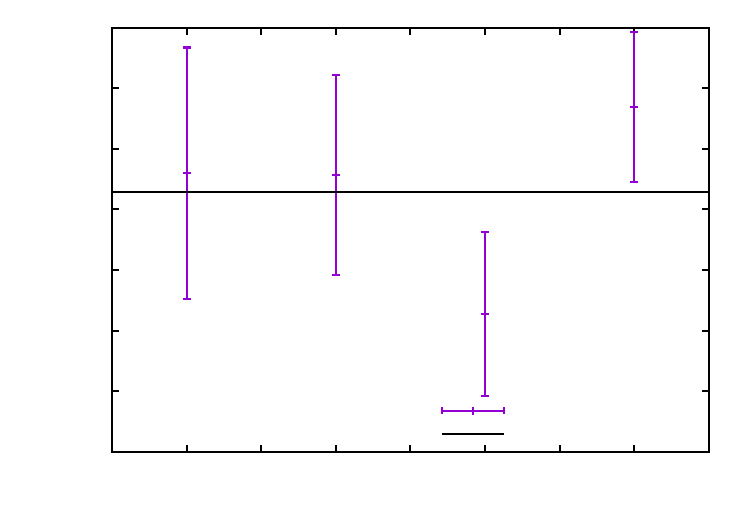
\includegraphics{gbesch}}%
    \gplfronttext
  \end{picture}%
\endgroup

	\caption{Bestimmung der Erdbeschleunigung bei verschiedenen Seillängen und Mittelwert der Messungen.}
	\label{fig:gbesch}
\end{figure}

Im zweiten Teil soll mit einem \textbf{Foucaultschen Pendel} die Erdrotation nachgewiesen werden.
Bei diesem Pendel handelt es sich um sehr langes und schweres Pendel, das lange pendeln kann.
Aufgrund der Corioliskraft dreht sich die Pendelrichtung, eigentlich dreht sich jedoch der Boden unter dem Pendel.
Dies kann man sich an den Polen gut vorstellen.
Dort ist diese Rotationsperiode $T=24\,$h.
Je näher man dem Äquator kommt, desto länger wird sie; da dort jedoch keine Corioliskraft wirkt, würde dort der Versuch nicht funktionieren.
In der Vorlesung wurde hergeleitet, dass für die Rotationsperiode 
\begin{align}
	T=\frac{24\,\si{\hour}}{\sin\phi}
	\label{eq:foucault}
\end{align}
gilt, wobei $\phi$ der Breitengrad ist.
Man lenkt das Pendel also aus und wartet eine gewisse Zeit, nach der man schaut, wie weit sich die Pendelebene gedreht hat.
Dies wird bei unserem Pendel durch Aufleuchten von LEDs in $1^\circ$-Schritten realisiert.
Die Messung ergab eine Drehung von $9^\circ$ in etwa $24\,$min.
Dies entspricht einer Rotationsperiode von $T=16\,$h, widerspricht somit \eqref{eq:foucault}.
Es muss sich also um einen Fehler im Aufbau handeln, welcher zu einer verstärkten Rotation oder einer Pendel-Vorzugsrichtung führt.
Dies geschieht etwa, wenn das Pendel etwas elliptisch schwingt.
Um dies zu verhindern, ist ganz oben der sog. Charron-Ring angebracht, an den sich das Stahlsein anschmiegen soll.
Bei der ersten Messung war der Ausschlag jedoch so gering, dass dieser nicht berührt wurde.
Deshalb ist der ganze Versuch mit dem maximal möglichen Ausschlag (ohne irgendwo anzuecken) wiederholt worden:
Diese Messung ergab eine Drehung von $26^\circ$ in etwa $100\,$min, also $T=\frac{360}{26}\cdot 100\,\si{min}\approx23\,$h.
Dieser Wert ist also etwas besser, jedoch sollte der Wert für Göttingen bei $T(\phi\approx 51.5^\circ)\approx30\,\si{\hour} \;40\,\si{\minute}$ liegen.
Es muss also noch weitere Messfehler geben.

\section{Erdumfang}
Eratosthenes konnte schon 200 v.Chr. den Erdumfang bestimmen:
Er stellte fest, dass die Sonne wenige Minuten am längsten Tag im Jahr in Syene, dem heutigen Assuan, keinen Schatten wirft, sie also genau über einem steht. Im nördlich gelegenen Alexandria jedoch beträgt der Schattenwurf $7^\circ12'$.
Die Luftlinie zwischen den beiden Orten beträgt etwa $840\,$km, jedoch sind sie nicht auf dem gleichen Längengrad. Man muss etwa $20^\circ$ von Assuan nach Westen gehen, um nach Alexandria zu gelangen.
So ist der Nord-Süd-Abstand der beiden Städte nur $\cos(20^\circ) \cdot 840\,$km$\,= 790\,$km.
Aus dem Schattenwurf kann man ableiten, dass dies der 50ste Teil des Erdumfangs sein muss.
Also beträgt der Erdumfang etwa $39500\,$km.
Bei einer Messung am Globus im DLR-SchoolLab beträgt der Winkel zwischen den beiden Städten etwa $8^\circ$.
So erhält man einen Erdumfang von etwa $\frac{360}{8} \cdot 840\,$km$\,=37800\,$km.
Da man aber den Winkel nicht sehr genau messen konnte, ist dieser Wert mit einer großen Ungenauigkeit behaftet.


Um nun die Strecke zwischen zwei Städten zu messen, schritten früher amtliche Schrittzähler diese mit einer Kette zwischen den Beinen ab.
Damit wurde die Schrittlänge konstant gehalten.
Wenn man nun um ein Hindernis laufen musste, lief man senkrecht zur eigentlichen Richtung, zählte diese Schritte nicht, lief ein Stück parallel  zur eigentlichen Richtung (Schritte werden gezählt), um dann wieder nicht zählend senkrecht zurück zulaufen.
Um sicherzustellen, dass man rechtwinklig zur bisherigen Route läuft, nutzt man z.B. ein an den Enden verknotetes Seil mit 12 Knoten, die in äquidistanten Abständen vorkommen.
Nun wird das Seil zu einem Dreieck mit den Kantenlängen $3,4\,$sowie$\,5$ gelegt, denn nach dem Satz von Pythagoras ist ein solches Dreieck rechtwinklig ($3^2+4^2=5^2$).
So kann man auch die Entfernung der obigen Städte in Nord-Süd-Richtung messen.

\end{document}
